\section{Mathematische Grundlagen}

\subsection{Trigonometrie}

% 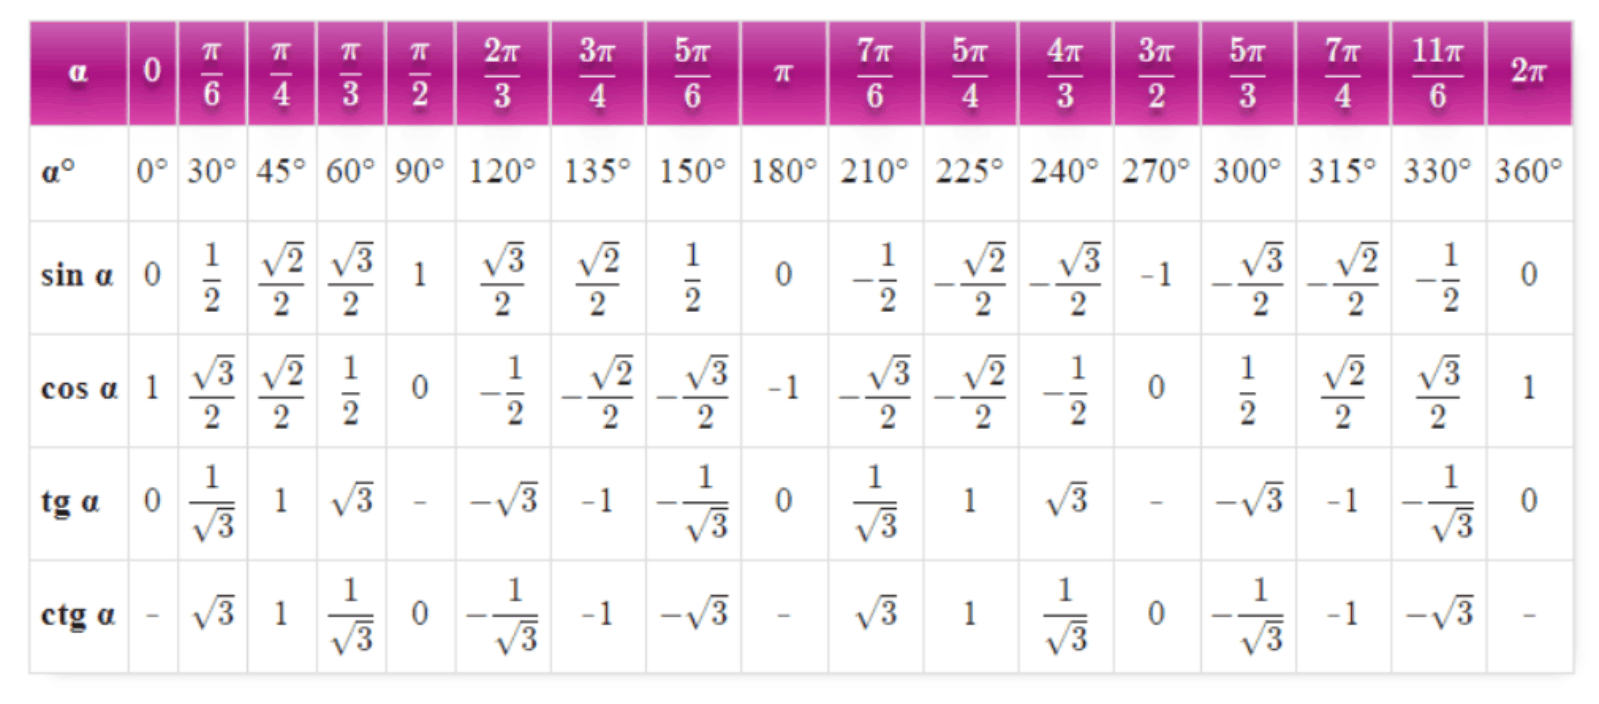
\includegraphics[width=\columnwidth]{images/trigo.png}

\begingroup
\renewcommand{\arraystretch}{2}
\setlength{\tabcolsep}{0mm}
\scalebox{0.33}{
\Huge
\begin{tabularx}{3\columnwidth}{rp{1mm}V{3}*{17}{C}}
    \rowcolor{subsectioncolor!30}$\bm{\alpha}$\phantom{${}^{\circ}$} && $0$ & $\dfrac{\pi}{6\mathstrut}$ & $\dfrac{\pi}{4}$ & $\dfrac{\pi}{3}$ & $\dfrac{\pi}{2}$ & $\dfrac{2\pi}{3}$ & $\dfrac{3\pi}{4}$ & $\dfrac{5\pi}{6}$ & $\pi$ & $\dfrac{7\pi}{6}$ & $\dfrac{5\pi}{4}$ & $\dfrac{4\pi}{3}$ & $\dfrac{3\pi}{2}$ & $\dfrac{5\pi}{3}$ & $\dfrac{7\pi}{4}$ & $\dfrac{11\pi}{6}$ & $2\pi$ \\\hline
    \rowcolor{subsectioncolor!30}$\bm{\alpha^\circ}$ && \phantom{${}^\circ$}$0^\circ$ & $30^\circ$ & $45^\circ$ & $60^\circ$ & $90^\circ$ & $120^\circ$ & $135^\circ$ & $150^\circ$ & $180^\circ$ & $210^\circ$ & $225^\circ$ & $240^\circ$ & $270^\circ$ & $300^\circ$ & $315^\circ$ & $330^\circ$ & $360^\circ$ \\\hline
    $\bm{\sin(\alpha)}$ && $0$ & $\dfrac{1}{2\mathstrut}$ & $\dfrac{\sqrt{2}}{2}$ & $\dfrac{\sqrt{3}}{2}$ & $1$ & $\dfrac{\sqrt{3}}{2}$ & $\dfrac{\sqrt{2}}{2}$ & $\dfrac{1}{2}$ & $0$ & $-\dfrac{1}{2}$ & $-\dfrac{\sqrt{2}}{2}$ & $-\dfrac{\sqrt{3}}{2}$ & $-1$ & $-\dfrac{\sqrt{3}}{2}$ & $-\dfrac{\sqrt{2}}{2}$ & $-\dfrac{1}{2}$ & $0$ \\\hline
    $\bm{\cos(\alpha)}$ && $1$ & $\dfrac{\sqrt{3}}{2\mathstrut}$ & $\dfrac{\sqrt{2}}{2}$ & $\dfrac{1}{2}$ & $0$ & $-\dfrac{1}{2}$ & $-\dfrac{\sqrt{2}}{2}$ & $-\dfrac{\sqrt{3}}{2}$ & $-1$ & $-\dfrac{\sqrt{3}}{2}$ & $-\dfrac{\sqrt{2}}{2}$ & $-\dfrac{1}{2}$ & $0$ & $\dfrac{1}{2}$ & $\dfrac{\sqrt{2}}{2}$ & $\dfrac{\sqrt{3}}{2}$ & $1$ \\\hline
    $\bm{\tan(\alpha)}$ && $0$ & $\dfrac{\sqrt{3}}{3\mathstrut}$ & $1$ & $\sqrt{3}$ & $\pm\infty$ & $-\sqrt{3}$ & $-1$ & $-\dfrac{\sqrt{3}}{3}$ & $0$ & $\dfrac{\sqrt{3}}{3}$ & $1$ & $\sqrt{3}$ & $\pm\infty$ & $-\sqrt{3}$ & $-1$ & $-\dfrac{\sqrt{3}}{3}$ & $0$ \\\hline
    $\bm{\cot(\alpha)}$ && $\pm\infty$ & $\sqrt{3}$ & $1$ & $\dfrac{\sqrt{3}}{3\mathstrut}$ & $0$ & $-\dfrac{\sqrt{3}}{3}$ & $-1$ & $-\sqrt{3}$ & $\pm\infty$ & $\sqrt{3}$ & $1$ & $\dfrac{\sqrt{3}}{3}$ & $0$ & $-\dfrac{\sqrt{3}}{3}$ & $-1$ & $-\sqrt{3}$ & $\pm\infty$ \\
\end{tabularx}}
\endgroup


\subsubsection{Beziehungen zwischen $\bm{\sin(x)}$ und $\bm{\cos(x)}$}

\renewcommand{\arraystretch}{1.3}
\begin{tabular}{ll}
    $\sin(-a) = -\sin(a)$                                           & $\cos(-a) = \cos(a)$                                              \\
    $\sin(\pi - a) = \sin(a)$                                       & $\cos(\pi -a) = - \cos(a)$                                        \\		
    $\sin(\pi + a) = -\sin(a)$                                      & $\cos(\pi + a) = - \cos(a)$                                       \\	
    $\sin(\frac{\pi}{2} - a) = \sin(\frac{\pi}{2} + a) = \cos(a)$   & $\cos(\frac{\pi}{2} - a) = - \cos(\frac{\pi}{2} + a) = \sin(a)$
\end{tabular}


\subsubsection{Additionstheoreme}

\begin{tabular}{l}
    $\sin(a \pm b) = \sin(a) \cdot \cos(b) \pm \cos(a) \cdot \sin(b)$           \\
    $\cos(a \pm b) = \cos(a) \cdot \cos(b) \mp \sin(a) \cdot \sin(b) $          \\
    $\tan(a \pm b) = \frac{\tan(a) \pm \tan(b)}{1 \mp \tan(a) \cdot \tan(b)}$
\end{tabular}


\subsubsection{Summen und Differenzen}

\begin{tabular}{l}
    $\sin(a) + \sin(b) = 2 \cdot \sin \big( \frac{a+b}{2} \big) \cdot \cos \big( \frac{a-b}{2} \big)$   \\
    $\sin(a) - \sin(b) = 2 \cdot \sin \big( \frac{a-b}{2} \big) \cdot \cos \big( \frac{a+b}{2} \big)$   \\
    $\cos(a) + \cos(b) = 2 \cdot \cos \big( \frac{a+b}{2} \big) \cdot \cos \big( \frac{a-b}{2} \big)$   \\
    $\cos(a) - \cos(b) = -2 \cdot \sin \big( \frac{a+b}{2} \big) \cdot \sin \big( \frac{a-b}{2} \big)$  \\
    $\tan(a) \pm \tan(b) = \frac{\sin(a \pm b)}{\cos(a) \cdot \cos(b)}$ 
\end{tabular}


\subsubsection{Produkte}

\begin{tabular}{l}
    $\sin(a) \cdot \sin(b) = \frac{1}{2} \big( \cos(a-b) - \cos(a+b) \big) $    \\
    $\cos(a) \cdot \cos(b) = \frac{1}{2} \big( \cos(a-b) + \cos(a+b) \big) $    \\	
    $\sin(a) \cdot \cos(b) = \frac{1}{2} \big( \sin(a-b) + \sin(a+b) \big) $ 
\end{tabular}

    
\subsubsection{Winkelvielfache und Halbwinkel}

\begin{tabular}{ll}
    $\sin(2a) = 2 \, \sin(a) \cdot \cos(a)$                                 & $\sin(3a) = 3 \, \sin(a) -4 \, \sin^3(a)$                                 \\
    $\sin(4a) = 8 \, \cos^3(a) \cdot \sin(a) - 4 \, \cos(a) \cdot \sin(a)$  & $\sin \big( \frac{a}{2} \big) = \sqrt{\frac{1}{2}(1-\cos(a))}$            \\
    \\
    $\cos(2a) = \cos^2(a) - \sin^2(a)$                                      & $\cos(3a) = 4 \, \cos^3(a) -3 \, \cos(a)$                                 \\
    $\cos(4a) = 8 \, \cos^4(a) - 8 \, \cos^2(a) + 1$                        & $\cos \big( \frac{a}{2} \big) = \sqrt{\frac{1}{2}(1+\cos(a))}$
\end{tabular}


\subsubsection{Potenzen}

\begin{tabular}{ll}
    $\sin^2(a) = \frac{1}{2}(1-\cos(2a))$                   & $\cos^2(a) = \frac{1}{2}(1+\cos(2a))$                 \\	
    $\sin^3(a) = \frac{1}{4}(3\, \sin(a) - \sin(3a))$       & $\cos^3(a) = \frac{1}{4}(\cos(3a) + 3 \, \cos(a)$     \\	
    $\sin^4(a) = \frac{1}{8}(\cos(4a) -4 \, \cos(2a) +3)$   & $\cos^4(a) = \frac{1}{8}(\cos(4a) +4 \, \cos(2a) +3)$ 	
\end{tabular}

\subsection{Komplexwertige Exponentialfunktion}

\subsubsection{Exponentialgesetze}

Die Exponentialgesetze bleiben in $\mathbb{C}$ für \myul{\textbf{ganzzahlige}} Exponenten erhalten!

\begin{tabular}{lll ll}
    $\e^a \cdot \e^b = \e^{a+b}$    & & $\e^a : \e^b = \e^{a-b}$    & & $a, \; b \in \mathbb{C}$    \\
    $(\e^a)^k = \e^{ka}$            & &                             & & $k \in \mathbb{Z}$
\end{tabular}


\subsubsection{Definition komplexwertige Exponentialfunktion}

\vspace{-0.2cm}
$$\crd{\e^z} = \e^{z_1 + jz_2} = \e^{z_1} \cdot \e^{j z_2} = \e^{z_1} \cdot \cjs(z_2)$$
Die koplexwertige Exponentialfunktion ist $2 \pi \jimg$-periodisch auf der $y$-Achse) 
    


\subsection{Partielle Integration}

\vspace{-0.2cm}
\begin{minipage}[c]{0.48\columnwidth}
    $$ \int f' \cdot g \, \diff x = f \cdot g - \int f \cdot g' \, \diff x $$
\end{minipage}
\hfill
\begin{minipage}[c]{0.48\columnwidth}
    $$ \int f \cdot g' \, \diff x  = f \cdot g - \int f' \cdot g \, \diff x $$
\end{minipage}


\subsection{Wichtige Ableitungen / Integrale}

\renewcommand{\arraystretch}{2}
\begin{tabular}{| c | c | c | c |}
    \hline
    $\bm{f'(t)}$                                                & $\bm{f(t)}$                           & $\bm{F(t)}$                   &               \\
    \hline
    $n \cdot \cos(n \, t)$                                      & $\sin(n \, t)$                        & $- \frac{\cos(n \, t)}{n}$    & $(n \neq 0)$  \\
    \hline     
    $- n \cdot \sin(n \, t)$                                    & $\cos(n \, t)$                        & $ \frac{\sin(n \, t)}{n}$     & $(n \neq 0)$  \\
    \hline
    \cbl{$ - \jimg \, \omega \, \e^{- \jimg \, \omega \, t}$}   & \cbl{$\e^{- \jimg \, \omega \, t}$}   & \cbl{$\frac{\e^{- \jimg \, \omega \, t}}{- \jimg \, \omega} = \frac{\jimg}{\omega} \e^{-\jimg \, \omega \, t}$} & \cbl{ $(n \neq 0)$ } \\
    \hline
\end{tabular}
\renewcommand{\arraystretch}{1}


\subsection[Einheitsprungfunktion ]{Einheitsprungfunktion $\sigma(t)$}

\begin{minipage}[c]{0.38\columnwidth}
    $$\sigma(t) = \begin{cases}			
    0           & \text{für} \; t < 0 \\
    \frac{1}{2} & \text{für} \; t = 0 \\ 
    1           & \text{für} \; t > 0 
\end{cases}$$
\end{minipage}
\hfill
\begin{minipage}[c]{0.5\columnwidth}
    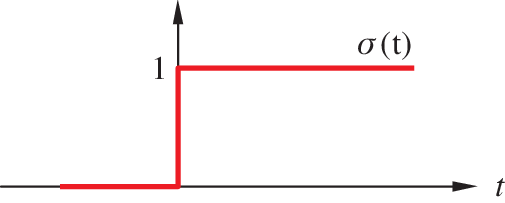
\includegraphics[width=\columnwidth]{images/einheitssprung.png}
\end{minipage}


\subsection{Polynomdivision}

Liefert Summe aus ganzrationaler Funktion und echt gebrochener Funktion.


\example{Polynomdivision}

\polylongdiv[style=C]{-2x^2-x-1}{x-1} 
    
    
\subsection{Partialbruchzerlegung}

\begin{tabular}{lll}
    (1)     & echt gebrochen ($m < n$)  \\
            & Ja: \textrightarrow\ (2)   & Nein: Polynomdivision \\
    (2)     & Nenner faktorisieren      \\
            & pro Faktor ein Teilbruch  \\
    (3)     & Berechnung Zählerkonstanten       \\
    (3.1)   & Gleichnahmig machen (kgV) \\
    (3.2)   & Zählergleichung           \\
    (3.3)   & Einsetzen von 'guten' $x$-Werten  \\			
\end{tabular}


\example{Partialbruchzerlegung}

\renewcommand{\arraystretch}{1.7}
\begin{tabular}{ll}
(1)     & $f(x) = \frac{1}{a^2 - x^2}$                                  \\
(2)     & $a^2 - x^2 = (a+x)(a-x)$                                      \\
(3)     & $\frac{A}{a+x} + \frac{B}{a-x} = \frac{1}{a^2 - x^2}$         \\
(3.1)   & $\frac{A(a-x) + B(a+x)}{a^2 - x^2} = \frac{1}{a^2 - x^2}$     \\
(3.2)   & $A(a-x) + B(a+x) = 1$                                         \\
(3.3)   & $x = a$ \textrightarrow\ $B(2a) = 1$ \textrightarrow\ $B = \frac{1}{2a}$    \\			
        & $x = -a$ \textrightarrow\ $A(2a) = 1$ \textrightarrow\ $A = \frac{1}{2a}$
\end{tabular}


\subsubsection{Spezielle Ansätze PBZ}

\renewcommand{\arraystretch}{2}
\begin{tabular}{ll}
    $f(x)$  & $ = \frac{5x^2-37x+54}{x^3-6x^2+9x} = \frac{A}{x}+\frac{B}{x-3}+\frac{C}{(x-3)^2} = \frac{A(x-3)^2+Bx(x-3)+Cx}{x(x-3)^2}$ \\ 
    $f(x)$  & $ = \frac{1.5x}{x^3-6x^2+12x-8} = \frac{A}{x-2}+\frac{B}{(x-2)^2}+\frac{C}{(x-2)^3 } =\frac{A(x-2)^2+B(x-2)+C}{(x-2)^3}$  \\
    $f(x)$  & $ = \frac{x^2-1}{x^3+2x^2-2x-12} = \frac{A}{x-2}+\frac{Bx+C}{x^2+4x+6} = \frac{A(x^2+4x+6)+(Bx+C)(x-2)}{(x-2)(x^2+4x+6)}$
\end{tabular}
\renewcommand{\arraystretch}{1}

